\documentclass{article}

\usepackage{minitoc}
\usepackage{tabularx}
\usepackage{booktabs}
\usepackage{graphicx}
\usepackage{hyperref}
\usepackage{xcolor}
\usepackage{blkarray}
\usepackage{amsthm, amssymb, amsmath}
\usepackage{caption}
\usepackage{subcaption}
\usepackage{multirow}
\usepackage[ruled,vlined]{algorithm2e}

\usepackage{natbib}
\bibliographystyle{abbrvnat}

\theoremstyle{definition}
\newtheorem{definition}{Definition}[section]
\newtheorem{theorem}{Theorem}[section]
\newtheorem{lemma}[theorem]{Lemma}
\newtheorem{conjecture}[theorem]{Conjecture}

\usepackage[margin=2.5cm, includefoot, footskip=30pt]{geometry}
\pagestyle{plain}
\setlength{\parindent}{0em}
\setlength{\parskip}{1em}

\renewcommand{\baselinestretch}{1}

\newcommand{\nikoleta}[1]{\textcolor{teal}{{\bf NG:} #1}}

\newtheorem{proposition}{Proposition}

\title{Good reactive strategies in the iterated prisoner's dilemma}

\author{Nikoleta E. Glynatsi, Christian Hilbe, Martin Nowak}
\date{}

\begin{document}

\maketitle

We consider the infinitely repeated prisoner's dilemmas with two players,
denoted as \(p\) and \(q\). At each turn, players \(p\) and \(q\) can choose to
cooperate (\(C\)) or to defect (\(D\)). A player who cooperates pays a cost \(c
> 0\) to provide a benefit \(b > c\) for the co-player. A cooperator either gets
\(b - c\) (if the co-player also cooperates) or \(-c\) (if the co-player
defects). Respectively, a defector either gets \(b\) (if the co-player
cooperates) or 0 (if the co-player defects). A strategy for player \(p\) is a
mapping from the entire history of play to an action of the prisoner's dilemma.
There are infinitely many strategies that \(p\) can choose from, however, it is
commonly assumed that the players' strategies depend on the last \(n\) turns
only. These strategies are called memory-\(n\) strategies.

\citep{akin:EGADS:2016} explores memory-1 strategies, and more specifically,
characterizes a subset of memory-one strategies called good.

The aim of this work is extend the result of~\citep{akin:EGADS:2016} to the case


For the iterated prisoner's dilemma
there are infinitely many strategies,

The aim of this work is to characterize all good Nash reactive strategies, with
memory two (\(n=2\)), in the infinitely repeated prisoner's dilemma. We refer to
these strategies as two-bit reactive strategies.

\section{Two-bits reactive strategies}

In the case of \(n=2\) there are 16 possible outcomes. We denote the possible
outcomes as \(E_p E_q | F_p F_q\) (\(E_p, E_q, F_p, F_q \in \{C, D\}\)) where
the outcome of the previous round is \(E_p E_q\) and the outcome of the current
round is \(F_p F_q\). With the outcomes listed in order as \(CC|CC, CC|CD,
\dots, DD|DC, DD|DD\)  a two-bit reactive strategy for \(p\) is a vector
\(\mathbf{p} = (p_1, p_2, p_1, p_2, p_3, p_4, p_3, p_4, p_1, p_2, p_1, p_2, p_3,
p_4, \allowbreak p_3, p_4)\) where \(p_1\) is the probability cooperating when
the last two actions of the co-player were \(C\) and \(C\), \(p_2\) is the
probability cooperating when the last two actions of the co-player were \(C\)
and \(D\), and so on. For simplicity, we denote a two-bit reactive strategy for
\(p\) as \(\mathbf{\hat{p}} = (\hat{p}_1, \hat{p}_2, \hat{p}_3, \hat{p}_4)\).

\begin{definition}
  We call a two-bit reactive strategy \textbf{agreeable} if it is never the
  first to defect, and if it always cooperates with a probability 1 if the
  co-player has consecutively cooperated in that last two rounds, thus \(\hat{p}_1=1\).
\end{definition}

The play between a pair of two-bit reactive strategies can be described by a
Markov process with the transition matrix \(M\).

% \resizebox{\linewidth}{!}{%
% $
% M = \left(\begin{array}{cccccccccccccccc}
%  \hat{p}_1 \hat{q}_1 & \hat{p}_1 (1-\hat{q}_1) & (1-\hat{p}_1) \hat{q}_1 & (1-\hat{p}_1) (1-\hat{q}_1) & 0 & 0 & 0 & 0 & 0 & 0 & 0 & 0 & 0 & 0 & 0 & 0 \\
%  0 & 0 & 0 & 0 & \hat{p}_2 \hat{q}_1 & \hat{p}_2 (1-\hat{q}_1) & (1-\hat{p}_2) \hat{q}_1 & (1-\hat{p}_2) (1-\hat{q}_1) & 0 & 0 & 0 & 0 & 0 & 0 & 0 & 0 \\
%  0 & 0 & 0 & 0 & 0 & 0 & 0 & 0 & \hat{p}_1 \hat{q}_2 & \hat{p}_1 (1-\hat{q}_2) & (1-\hat{p}_1) \hat{q}_2 & (1-\hat{p}_1) (1-\hat{q}_2) & 0 & 0 & 0 & 0 \\
%  0 & 0 & 0 & 0 & 0 & 0 & 0 & 0 & 0 & 0 & 0 & 0 & \hat{p}_2 \hat{q}_2 & \hat{p}_2 (1-\hat{q}_2) & (1-\hat{p}_2) \hat{q}_2 & (1-\hat{p}_2) (1-\hat{q}_2) \\
%  \hat{p}_3 \hat{q}_1 & \hat{p}_3 (1-\hat{q}_1) & (1-\hat{p}_3) \hat{q}_1 & (1-\hat{p}_3) (1-\hat{q}_1) & 0 & 0 & 0 & 0 & 0 & 0 & 0 & 0 & 0 & 0 & 0 & 0 \\
%  0 & 0 & 0 & 0 & \hat{p}_4 \hat{q}_1 & \hat{p}_4 (1-\hat{q}_1) & (1-\hat{p}_4) \hat{q}_1 & (1-\hat{p}_4) (1-\hat{q}_1) & 0 & 0 & 0 & 0 & 0 & 0 & 0 & 0 \\
%  0 & 0 & 0 & 0 & 0 & 0 & 0 & 0 & \hat{p}_3 \hat{q}_2 & \hat{p}_3 (1-\hat{q}_2) & (1-\hat{p}_3) \hat{q}_2 & (1-\hat{p}_3) (1-\hat{q}_2) & 0 & 0 & 0 & 0 \\
%  0 & 0 & 0 & 0 & 0 & 0 & 0 & 0 & 0 & 0 & 0 & 0 & \hat{p}_4 \hat{q}_2 & \hat{p}_4 (1-\hat{q}_2) & (1-\hat{p}_4) \hat{q}_2 & (1-\hat{p}_4) (1-\hat{q}_2) \\
%  \hat{p}_1 \hat{q}_3 & \hat{p}_1 (1-\hat{q}_3) & (1-\hat{p}_1) \hat{q}_3 & (1-\hat{p}_1) (1-\hat{q}_3) & 0 & 0 & 0 & 0 & 0 & 0 & 0 & 0 & 0 & 0 & 0 & 0 \\
%  0 & 0 & 0 & 0 & \hat{p}_2 \hat{q}_3 & \hat{p}_2 (1-\hat{q}_3) & (1-\hat{p}_2) \hat{q}_3 & (1-\hat{p}_2) (1-\hat{q}_3) & 0 & 0 & 0 & 0 & 0 & 0 & 0 & 0 \\
%  0 & 0 & 0 & 0 & 0 & 0 & 0 & 0 & \hat{p}_1 \hat{q}_4 & \hat{p}_1 (1-\hat{q}_4) & (1-\hat{p}_1) \hat{q}_4 & (1-\hat{p}_1) (1-\hat{q}_4) & 0 & 0 & 0 & 0 \\
%  0 & 0 & 0 & 0 & 0 & 0 & 0 & 0 & 0 & 0 & 0 & 0 & \hat{p}_2 \hat{q}_4 & \hat{p}_2 (1-\hat{q}_4) & (1-\hat{p}_2) \hat{q}_4 & (1-\hat{p}_2) (1-\hat{q}_4) \\
%  \hat{p}_3 \hat{q}_3 & \hat{p}_3 (1-\hat{q}_3) & (1-\hat{p}_3) \hat{q}_3 & (1-\hat{p}_3) (1-\hat{q}_3) & 0 & 0 & 0 & 0 & 0 & 0 & 0 & 0 & 0 & 0 & 0 & 0 \\
%  0 & 0 & 0 & 0 & \hat{p}_4 \hat{q}_3 & \hat{p}_4 (1-\hat{q}_3) & (1-\hat{p}_4) \hat{q}_3 & (1-\hat{p}_4) (1-\hat{q}_3) & 0 & 0 & 0 & 0 & 0 & 0 & 0 & 0 \\
%  0 & 0 & 0 & 0 & 0 & 0 & 0 & 0 & \hat{p}_3 \hat{q}_4 & \hat{p}_3 (1-\hat{q}_4) & (1-\hat{p}_3) \hat{q}_4 & (1-\hat{p}_3) (1-\hat{q}_4) & 0 & 0 & 0 & 0 \\
%  0 & 0 & 0 & 0 & 0 & 0 & 0 & 0 & 0 & 0 & 0 & 0 & \hat{p}_4 \hat{q}_4 & \hat{p}_4 (1-\hat{q}_4) & (1-\hat{p}_4) \hat{q}_4 & (1-\hat{p}_4) (1-\hat{q}_4) \\
% \end{array}\right).$}

The invariant distribution \(\mathbf{v}\) is the solution to
\(\mathbf{v} M = \mathbf{v}\). We define expected payoffs,
denoted as \(\mathbf{s}_{p} \text{ and } \mathbf{s}_{q}\),
based on the outcome of the last round. Thus,

\begin{equation*}
    \mathbf{s}_{p} = \mathbf{v} \cdot \mathbf{S}_{p} \quad \text{ and } \quad \mathbf{s}_{q} = \mathbf{v} \cdot \mathbf{S}_{q}.
\end{equation*}

where

\begin{equation}\label{eq:last_round_two_bits}
  \begin{array}{*{16}{c}}
    \mathbf{S}_{p} = ( b\!-\!c , & -c , & b , & 0 , & b\!-\!c , & -c , & b , & 0 , & b\!-\!c , & -c , & b , & 0 , & b\!-\!c , & -c , & b , & 0)  \;, \\
    \mathbf{S}_{q} = ( b\!-\!c, & b, & -c, & 0, & b\!-\!c, & b, & -c, & 0, & b\!-\!c, & b, & -c, & 0, & b\!-\!c, & b, & -c, & 0),
  \end{array}
\end{equation}

and \(b > c > 0\).

From~\citep{akin:EGADS:2016}, a strategy for \(p\) is called \textbf{good} if
(i) it is agreeable, and (ii) if for any general strategy chosen by \(q\)
against it the expected payoffs satisfy:

\begin{equation}
    s_{\mathbf{q}} \geq b\!-\!c \qquad \Rightarrow \qquad s_{\mathbf{q}} = s_{\mathbf{p}} =  b\!-\!c,
\end{equation}

and the strategy is of \textbf{Nash type} if (i) it is agreeable and (ii)
if the expected payoffs against any general strategy used by \(q\) satisfy:

\begin{equation}
    s_{\mathbf{q}} \geq b\!-\!c \qquad \Rightarrow \qquad s_{\mathbf{q}} =  b\!-\!c.
\end{equation}

Hence, a strategy is good if the co-player achieves the reward payoff if and
only if the focal player does as well, and a Nash type strategy reassures that
the co-player can never receive a payoff higher than \(b\!-\!c\) (the payoff for
mutual cooperation).

\citep{akin:EGADS:2016} derives an interesting relationship between a player's
memory-one strategy (Theorem 1.3) and the resulting invariant distribution of the repeated
game. This relationship allows him to characterize all memory-one strategies
that are of \textit{Nash type} and \textit{good}. In order to characterize all two-bit reactive strategies that are good we
initially extend Theorem 1.3 from~\citep{akin:EGADS:2016} to two-bit reactive
strategies (Lemma~\ref{lemma:akin_extended}). 
We then use Lemma~\ref{lemma:akin_extended} to prove
Theorem~\ref{theorem:two_bit_nash_and_good}.

\begin{lemma}\label{lemma:akin_extended}
  Assume that player \(p\) uses a two-bit reactive strategy \(\mathbf{\hat{p}}\),
  and \(q\) uses a strategy that leads to a sequence
  of distributions \(\{\mathbf{v}^{(n)}, n = 1, 2, ...\}\) with
  \(\mathbf{v}^{(k)}\) representing the distribution over the states in the
  \(k^{\text{th}}\) round of the game. Let \(\mathbf{v}\) be the associated
  stationary distribution, and let \(\mathbf{\tilde{p}} = \mathbf{\hat{p}} - \mathbf{\hat{e}}_{1 2}\)
  where \(\mathbf{\hat{e}}_{1 2} = (1, 1, 1, 1, \allowbreak 0,
  0, 0, 0, 1, 1, 1, 1, 0, 0, 0, 0)\). Then,

  \begin{align*}
    \lim_{n \rightarrow \infty} \frac{1}{n} \sum_{k=1}^{n} \mathbf{v}^{(k)} \cdot\mathbf{\tilde{p}} & = 0, \text{ and therefore } \mathbf{v} \cdot \mathbf{\tilde{p}} = 0.
  \end{align*}

  \begin{align}\label{eq:akin_extended}
  \mathbf{v}^{(n)} \cdot \mathbf{\tilde{p}} = 0 \Rightarrow & \nonumber \\
  & (v_{1} + v_{9}) (1 - \hat{p}_1) + (v_{2} + v_{10}) (1 - \hat{p}_2)  + (v_{5} + v_{13}) (1 - \hat{p}_3) + (v_{6} + v_{14}) (1 - \hat{p}_4) \nonumber \\
  & + (v_{3} + v_{11})\hat{p}_1  + (v_{4} + v_{12})\hat{p}_2 + (v_{7} + v_{15}) \hat{p}_3 + (v_{8} + v_{16}) \hat{p}_4 = 0.
  \end{align}
\end{lemma}

\begin{proof}
The probability that \(p\) cooperates in the \(n^{\text{th}}\) round, denoted
by \(v_{\text{C}}^{(n)}\), is \(v_{\text{C}}^{(n)} = v_{1}^{(n)} +
v_{2}^{(n)} + v_{5}^{(n)} + v_{6}^{(n)} + v_{9}^{(n)} +  v_{10}^{(n)} +
v_{13}^{(n)} + v_{14}^{(n)} = v \cdot \mathbf{\hat{e}}_{1 2}\)
where \(\mathbf{\hat{e}}_{1 2} = (1, 1, 1, 1, \allowbreak 0,
0, 0, 0, 1, 1, 1, 1, 0, 0, 0, 0)\). The probability that \(p\) cooperates in the \((n + 1)^{th}\) round, denoted
by \(v_{\text{C}}^{(n + 1)}\) = \(v^{(n)} \cdot \mathbf{\hat{p}}\).
Hence,

\begin{equation*}
v_{\text{C}}^{(n + 1)} - v_{\text{C}}^{(n)} = \mathbf{v^{(n)}} \cdot \mathbf{\hat{p}} - v \cdot \mathbf{\hat{e}}_{1 2}
= \mathbf{v^{(n)}} \cdot (\mathbf{\hat{p}} - \mathbf{\hat{e}}_{1 2}) = v^{(n)} \cdot \mathbf{\tilde{p}}.
\end{equation*}

This implies,

\begin{equation}
\sum^{n}_{k=1} v^{(k)} \cdot \mathbf{\tilde{p}} = \sum^{n}_{k=1} v_{\text{C}}^{(k + 1)} - v_{\text{C}}^{(k)} \quad \Rightarrow \quad \sum^{n}_{k=1} v^{(k)} \cdot \mathbf{\tilde{p}} =  v_{\text{C}}^{(n + 1)} - v_{\text{C}}^{(1)}.
\end{equation}

As the right side has absolute value at most 1,

\begin{equation}
\lim_{n \rightarrow \infty} \frac{1}{n} \sum^{n}_{k=1} v^{(k)} \cdot \mathbf{\tilde{p}} = 0. 
\end{equation}

\end{proof}

\begin{theorem}\label{theorem:two_bit_nash_and_good}
    Let the two-bit reactive strategy \(\mathbf{\hat{p}} = (\hat{p}_{1}, \hat{p}_{2}, \hat{p}_{3}, \hat{p}_{4})\) be an \textbf{agreeable
    strategy}; that is \(\hat{p}_1 = 1\). Strategy \(\mathbf{\hat{p}}\) is \textbf{Nash} if the
    following inequalities hold:
    \begin{equation*}
        \hat{p}_4 \leq 1 - \frac{c}{b} \qquad  \hat{p}_2  \leq \hat{p}_4 \qquad \hat{p}_3 \leq 1 \qquad 1 + \hat{p}_2 \leq \frac{b}{c} - \hat{p}_4 \frac{b\!-\!c}{c}
    \end{equation*}
    
    The agreeable strategy \(\mathbf{\hat{p}}\) is good if the inequalities above are strict.
    \end{theorem}
    
    \begin{proof}
    We first eliminate the possibility \(\hat{p}_4 = 1\). If \(\hat{p}_4 = 1\),
    then \(\mathbf{\hat{p}} = (1, \hat{p}_2, \hat{p}_3, 1)\). If against this
    \(q\) plays AllD \(= (0, 0, 0, 0)\), then \(v_6 = 1\). So the strategies
    end up in the outcome \(CD|CD\) with  with \(s_\mathbf{q} = b\) and
    \(s_\mathbf{p} = -c\). Hence, \(\mathbf{\hat{p}}\) is not of Nash type.

    We now assume \(1 - \hat{p}_4 > 0\). Observe that
    
    \begin{align}\label{eq:nash_condition_last_round}
    s_\mathbf{q} - (b\!-\!c) & = \mathbf{v} \times \mathbf{S}_{q} - (b\!-\!c) \sum_{i=1}^{16} v_{i}\\ \nonumber
    & = (v_{2} + v_{6} + v_{10} + v_{14}) c + (c - b) (v_{4} + v_{8} + v_{12} + v_{16}) - b (v_{3} + v_{7} + v_{11} + v_{15}) .
    \end{align}
    
    Multiplying by the positive quantity \((1 - \hat{p}_4)\) and collecting terms, we have
    
    \begin{align}
    s_\mathbf{q} - (b\!-\!c)\geq 0 & \Rightarrow \\ \nonumber
    (1 - \hat{p}_4)(v_{6} + v_{14}) c & \geq  - c(1 - \hat{p}_4)(v_{2} + v_{10}) + (1 - \hat{p}_4)(-c + b) (v_{4} + v_{8} + v_{12} + v_{16}) + b (1 - \hat{p}_4) (v_{3} + v_{7} + v_{11} + v_{15}) .
    \end{align}
    
    Since \(\tilde{p_1} = 0\), equation (\ref{eq:akin_extended}) implies
    
    \[(1 - \hat{p}_2)
    (v_{10} + v_{2}) + (1 - \hat{p}_3) (v_{13} + v_{5}) +  (1 - \hat{p}_4) (v_{14} + v_6)
    - \hat{p}_2 (v_{12} + v_4) - \hat{p}_3 (v_{15} + v_7) - \hat{p}_4 (v_{16} + v_{8}) - v_{11} - v_{3} = 0,\]
    and so,
    \[(1 - \hat{p}_4) (v_{14} + v_6) = - ((1 - \hat{p}_2)
    (v_{10} + v_{2}) + (1 - \hat{p}_3) (v_{13} + v_{5}) 
    - \hat{p}_2 (v_{12} + v_4) - \hat{p}_3 (v_{15} + v_7) - \hat{p}_4 (v_{16} + v_{8}) - v_{11} - v_{3}).\]
    
    Substituting this in the above inequality and collecting terms we get,
    
    \begin{align}
    & A (v_{10} + v_{2}) + B (v_{12} + v_4) 
    + C (v_{13} + v_5) + D (v_{15} + v_7) + E (v_{11} + v_{16} + v_3 + v_8) \geq  0 \label{eq:nash_condition_special_case} \\ \text{ with } \nonumber \\ 
    & \qquad A = c (\hat{p}_2 - \hat{p}_4), \qquad B = c (1 + \hat{p}_2 - \hat{p}_4) + b (-1 + \hat{p}_4), \qquad C = c (-1 + \hat{p}_3),  \nonumber \\
    & \qquad  \qquad  \qquad \qquad \qquad D = c \hat{p}_3 + b (-1 + \hat{p}_4), \qquad E = c + 
    b (-1 + \hat{p}_4). \nonumber
    \end{align}
    
    In the case where \(A, B, C, D\) and \(E\) are strictly smaller than 0, condition
    (\ref{eq:nash_condition_special_case}) holds iff \(v_2, v_3,
    v_4, v_5, v_7, v_8, v_{10},
    v_{11}, \allowbreak v_{12}, v_{13}, v_{15}, v_{16} =
    0\). This implies, that \((v_1 + v_9) (1 - \hat{p}_1) + (v_6 +
    v_{14}) (1 - \hat{p}_4) = 0\). \(\hat{p}_4\) can not be 1, thus \(v_6,
    v_{14} = 0\). This means \((v_1 + v_9) = 1\), so both
    players receive the reward payoff and \(\mathbf{\hat{p}}\) is good.
    
    For \(A, B, C, D, E \leq 0\) we derive the following conditions,
    
    \begin{align}\label{eq:nash_conditions}
    \hat{p}_4       & \leq 1 - \frac{c}{b} \\
    \hat{p}_2       & \leq \hat{p}_4 \\
    \hat{p}_3       & \leq 1 \\
    1 + \hat{p}_2 & \leq \frac{b}{c} - \hat{p}_4 \cdot \frac{b\!-\!c}{c}
    \end{align}
\end{proof}

\subsection{Numerical Evaluation}

To verify the result of Theorem~\ref{theorem:two_bit_nash_and_good} we explored
which agreeable strategies are Nash numerically. Namely, for a given agreeable
two-bit strategy, and we checked if condition \(\pi({\mathbf{q}},
\mathbf{\hat{p}}) \leq (b\!-\!c)\) was satisfied against all pure memory-two
strategies (\(\mathbf{q} \in \{0, 1\}^{16}\)). We recorded if the strategy was
Nash or not, and against which the pure strategies the condition for Nash was
not satisfied. We repeated this step for 10,000 random strategies, for parameter
values (\(b=2 \text{ and } c=1\)). The results are shown in
Figure~\ref{fig:two_bit_reactive_nash_results}. From
Figure~\ref{fig:two_bit_reactive_nash_results}\textbf{B)} we can conclude that
the inequalities~(\ref{eq:nash_conditions}) are sufficient for a point to be
Nash but not necessary.

Since a two-bit reactive strategy \(\mathbf{\hat{p}} = (\hat{p}_{1},
\hat{p}_{2}, \hat{p}_{3}, \hat{p}_{4})\) can only be a Nash equilibrium if {\it no} other strategy yields a larger payoff,  in particular neither \text{AllD} nor the \text{Alternator} strategy must yield a larger payoff, where
AllD\(=(0, 0, 0, 0, 0, 0, 0, 0, 0, 0, 0, 0, 0, 0, 0, 0)\) and
Alternator\(=(0, 0, 1, 1, 0, 0, 1, 1, 0, 0, 1, 1, 0, 0, 1, 1)\). 
We conclude that an agreeable two-bit reactive strategy  \(\mathbf{\hat{p}} = (\hat{p}_{1}, \hat{p}_{2}, \hat{p}_{3}, \hat{p}_{4})\) can only form a Nash equilibrium if 

\begin{align*}
\pi(\text{AllD}, \mathbf{\hat{p}}) \leq b\!-\!c & \quad \text{ and } \quad \pi(\text{Alternator}, \mathbf{\hat{p}}) \leq b\!-\!c,
\end{align*}
or equivalently, if
\begin{align}\label{Eq:NashConditionDonationGame}
  \hat{p}_4 \leq 1 - \frac{c}{b} & \quad \text{ and } \quad  \hat{p}_2 + \hat{p}_3 \leq 1 + \frac{b\!-\!c}{c}
\end{align}

In fact, a further numerical analysis suggests the following stronger result. 

\begin{conjecture}\label{conjecture:nash_from_numerical_results}
An agreeable two-bit reactive strategy \(\mathbf{\hat{p}} = (\hat{p}_{1}, \hat{p}_{2}, \hat{p}_{3}, \hat{p}_{4})\) is of Nash type if and only if conditions \eqref{Eq:NashConditionDonationGame} hold. 
\end{conjecture}

\begin{figure}[!htbp]
  \centering
  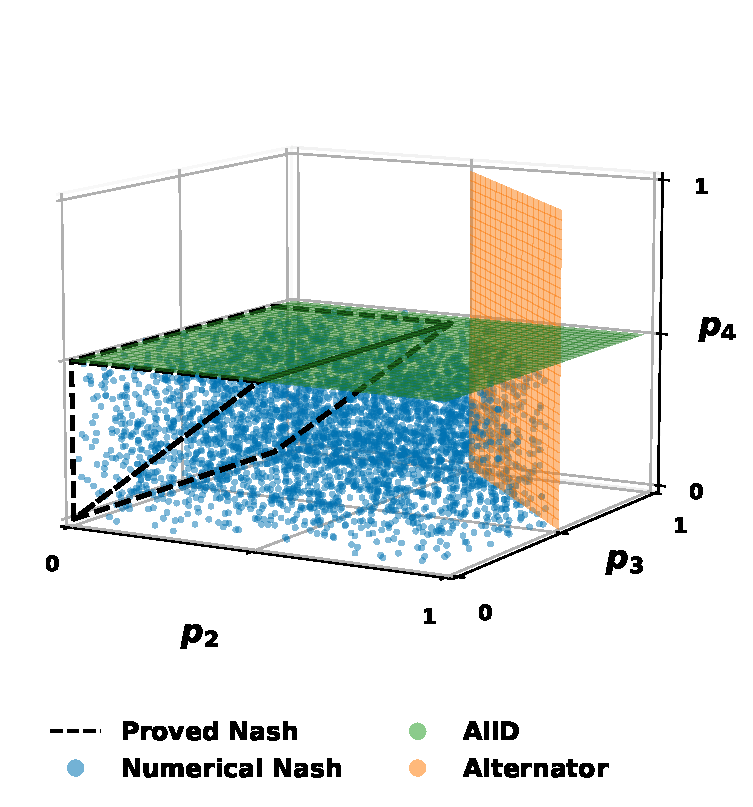
\includegraphics[width=.35\textwidth]{static/for_akin.pdf}
  \caption{\textbf{Nash results for two-bit strategies.}
  \textbf{A) Proved Nash.} We have shown that if a two-bit reactive
  strategy is within this space, thus satisfies conditions
  (\ref{eq:nash_conditions}), then it is good Nash. \textbf{B) Numerical Nash
  results.} The results from the numerical evaluation. We evaluated \(10 ^ 4\) points in
  the space. The numerical results have shown that there are two pure
  strategies that constrain the Nash space; these are AllD and Alternator.
  The equations for the planes are obtained by solving
  \(\pi(\mathbf{q}, \mathbf{\hat{p}}) = (b\!-\!c)\). The equations are
  \(\hat{p}_4 = 1 - \frac{c}{b} \text{ and }  \hat{p}_3 = 1 + \frac{b\!-\!c}{c} - \hat{p}_2\).
  Parameters: \(c=1, b=2\). \textbf{C) Numerical Nash for high benefit.} We repeat
  the numerical analysis for a higher value of benefit
  (\(b=7\)) for \(10 ^ 3\) random points. We can see that the strategies AllD
  and Alternator still constrain the space of possible Nash. Note that we do
  not plot \(\hat{p}_1\) for any of the above plots, since \(\hat{p}_1=1\).
  }\label{fig:two_bit_reactive_nash_results}
\end{figure}

\bibliography{bibliography.bib}

\end{document}